\begin{figure}[htp]
	\begin{center}
	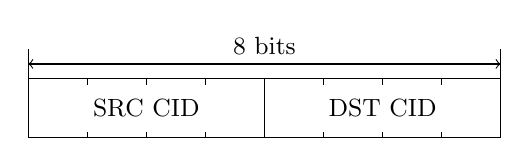
\begin{tikzpicture}[scale=0.75]
		\draw (0,0) rectangle (8,1);
		\draw (0,1) -- ++(0,0.5);
		\draw (8,1) -- ++(0,0.5);
		\draw[<->] (0,1.25) -- (8,1.25) node[midway, above] {\small 8 bits};

		\foreach \x in {1,2,...,7}{
			\draw (\x,1) -- ++(0,-0.1);
			\draw (\x,0) -- ++(0,0.1);
		}

		\draw (4,0) -- ++(0,1);
		\node at (2, 0.5) {\small SRC CID};
		\node at (6, 0.5) {\small DST CID};
	\end{tikzpicture}
	\end{center}
	\caption{Context ID Format}
	\label{fig:6lo_cid}
\end{figure}